Let,
\begin{align}
\vec{A}=\myvec{5 \\ -2}, \vec{B}=\myvec{6 \\ 4}, \vec{C}=\myvec{7 \\ -2 }\label{aug/2/5/eq:2.5.2}
\end{align}
% For the triangle to be isosceles triangle, one of\\
% \begin{align}
% 	\norm{\vec{A} - \vec{B}} =  \norm{\vec{B} - \vec{C}} \label{aug/2/5/eq:2.5.3}\\
% 	or \norm{\vec{A} - \vec{B}} =  \norm{\vec{B} - \vec{C}} \label{aug/2/5/eq:2.5.4}\\
% 	or \norm{\vec{B} - \vec{C}} =  \norm{\vec{C} - \vec{A}} \label{aug/2/5/eq:2.5.5}\\
% 	or \norm{\vec{C} - \vec{A}} =  \norm{\vec{A} - \vec{B}} \label{aug/2/5/eq:2.5.6}
% \end{align}
% Now,\\
\begin{align}
	% \vec{A-B} = \myvec{5-6 \\ (-2)-4} = \myvec{-1 \\ -6} \label{aug/2/5/eq:2.5.7}\\
 \norm{\vec{A-B}}^{2} = (-1)^{2}+(-6)^{2} = 37 \label{aug/2/5/eq:2.5.8}\\
% \vec{B-C} = \myvec{6-7 \\ 4-(-2)} = \myvec{-1 \\ 6} \label{aug/2/5/eq:2.5.9}\\
 \norm{\vec{B-C}}^{2} = (-1)^{2}+6^{2} = 37 \label{aug/2/5/eq:2.5.10}\\
% \vec{C-A} = \myvec{7-5 \\ (-2)-(-2) = \myvec{2 \\ 0}} \label{aug/2/5/eq:2.5.11}\\
% \implies \norm{\vec{C-A}}^{2} = 2^{2} = 4 \label{aug/2/5/eq:2.5.12}
\implies AB = BC
\end{align}
 
%  As 
% \begin{align}
% 	 \norm{\vec{A-B}}^{2} = \norm{\vec{B-C}}^{2} = 37 \label{aug/2/5/eq:2.5.13}
% \end{align}
% (From \eqref{aug/2/5/eq:2.5.8} and \eqref{aug/2/5/eq:2.5.10})\\
%  $\implies$ In $\Delta ABC$ sides $AB, BC$ are equal.\\
%  $\implies$ 
Hence, $\triangle ABC$ is isosceles.
 See Fig. 
%  You can also see fom the below diagram that the triangle is an isosceles triangle with sides $AB, BC$ equal.  \ref{aug/2/5/fig:2.5}

 
 \begin{figure}[h]
 	\centering
 	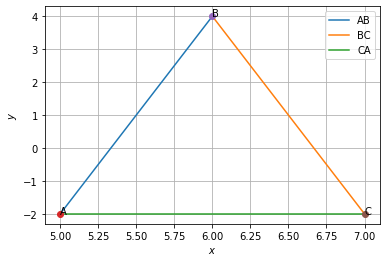
\includegraphics[width=\columnwidth]{solutions/aug/2/5/FIGURE-1.png}
 	\caption{$\Delta ABC$}
 	\label{aug/2/5/fig:2.5}
 \end{figure}
